\section{Пример III}

\subsection{Постановка задачи}
\renewcommand{\labelenumi}{\arabic{enumi})}
Задана ЗЛП:
\begin{equation}
	F(\vec{X}) = 3x_1 + 3x_2 \to max,
\end{equation}

\begin{equation}
\begin{cases}
x_1 - 4x_2 \le 4 \\
3x_1 + 2x_2 \le 6 \\
x_1 + 2x_2 \ge 2 \\
x_1, x_2 \ge 0 \\
\end{cases}
\end{equation}.

Необходимо:
\begin{enumerate}
\item Привести исходную ЗЛП к каноническому виду и решить методом искусственного базиса;
\item Решить исходную ЗЛП графически;
\end{enumerate}

\subsection{Решение исходной ЗЛП методом искусственного базиса}
Введем искусственные переменные и приведем к каноническому виду.
Для нахождения максимума, умножим целевую функцию на -1.

$$-F(\vec{X}) = -(-3x_1-3x_2+Wx_6) \to max$$
\begin{equation}
\label{cannonical}
\begin{cases}
x_1-4x_2+x_3=4\\
3x_1+2x_2+x_4=6\\
x_1+2x_2-x_5+ s_6=2\\
x_i, s_i \ge 0 \\
\end{cases}
\end{equation}

\begin{center}
\begin{tabular*}{\textwidth}{@{\extracolsep{\fill}}|c|c|c|c|c|c|c|c|c|c|c|}
\hline
$i$ & Базис & $C_i$ & B & $C_1 = -3$ & $C_2 = -3$ & $C_3 = 0$ & $C_4 = 0$ & $C_5 = 0$ & $C_6 = W$ & $\Theta_i$ \\
\hline
$1$ & $P_3$ & $0$ & $4$ & $1$ & $-4$ & $1$ & $0$ & $0$ & $0$ & --\\
$2$ & $P_4$ & $0$ & $6$ & $3$ & $2$ & $0$ & $1$ & $0$ & $0$ & $3$\\
$3$ & $P_6$ & W & $2$ & $1$ & $2$ & $0$ & $0$ & $-1$ & $1$ & $1$\\
\hline
$m+1$ & ~ & ~ & $0$ & $3$ & $3$ & $0$ & $0$ & $0$ & $0$ & ~ \\
\hline
$m+2$ & ~ & ~ & $2W$ & $1W$ & $2W$ & $0W$ & $0W$ & $-1W$ & $0W$ & ~ \\
\hline
\end{tabular*}
\end{center}
\begin{center}
\begin{tabular*}{\textwidth}{@{\extracolsep{\fill}}|c|c|c|c|c|c|c|c|c|c|c|}
\hline
$i$ & Базис & $C_i$ & B & $C_1 = -3$ & $C_2 = -3$ & $C_3 = 0$ & $C_4 = 0$ & $C_5 = 0$ & $C_6 = W$ & $\Theta_i$ \\
\hline
$1$ & $P_3$ & $0$ & $8$ & $3$ & $0$ & $1$ & $0$ & $-2$ & $2$ & $2,667$\\
$2$ & $P_4$ & $0$ & $4$ & $2$ & $0$ & $0$ & $1$ & $1$ & $-1$ & $2$\\
$3$ & $P_2$ & $-3$ & $1$ & $0,5$ & $1$ & $0$ & $0$ & $-0,5$ & $0,5$ & $2$\\
\hline
$m+1$ & ~ & ~ & $-3$ & $1,5$ & $0$ & $0$ & $0$ & $1,5$ & $-1,5$ & ~ \\
\hline
$m+2$ & ~ & ~ & $0W$ & $0W$ & $0W$ & $0W$ & $0W$ & $0W$ & $-1W$ & ~ \\
\hline
\end{tabular*}
\end{center}
\begin{center}
\begin{tabular*}{\textwidth}{@{\extracolsep{\fill}}|c|c|c|c|c|c|c|c|c|c|c|}
\hline
$i$ & Базис & $C_i$ & B & $C_1 = -3$ & $C_2 = -3$ & $C_3 = 0$ & $C_4 = 0$ & $C_5 = 0$ & $C_6 = W$ & $\Theta_i$ \\
\hline
$1$ & $P_3$ & $0$ & $2$ & $0$ & $0$ & $1$ & $-1,5$ & $-3,5$ & $3,5$ & --\\
$2$ & $P_1$ & $-3$ & $2$ & $1$ & $0$ & $0$ & $0,5$ & $0,5$ & $-0,5$ & $4$\\
$3$ & $P_2$ & $-3$ & $0$ & $0$ & $1$ & $0$ & $-0,25$ & $-0,75$ & $0,75$ & --\\
\hline
$m+1$ & ~ & ~ & $-6$ & $0$ & $0$ & $0$ & $-0,75$ & $0,75$ & $-0,75$ & ~ \\
\hline
$m+2$ & ~ & ~ & $0W$ & $0W$ & $0W$ & $0W$ & $0W$ & $0W$ & $-1W$ & ~ \\
\hline
\end{tabular*}
\end{center}
\begin{center}
\begin{tabular*}{\textwidth}{@{\extracolsep{\fill}}|c|c|c|c|c|c|c|c|c|c|c|}
\hline
$i$ & Базис & $C_i$ & B & $C_1 = -3$ & $C_2 = -3$ & $C_3 = 0$ & $C_4 = 0$ & $C_5 = 0$ & $C_6 = W$ & $\Theta_i$ \\
\hline
$1$ & $P_3$ & $0$ & $16$ & $7$ & $0$ & $1$ & $2$ & $0$ & $0$ & --\\
$2$ & $P_5$ & $0$ & $4$ & $2$ & $0$ & $0$ & $1$ & $1$ & $-1$ & $4$\\
$3$ & $P_2$ & $-3$ & $3$ & $1,5$ & $1$ & $0$ & $0,5$ & $0$ & $0$ & --\\
\hline
$m+1$ & ~ & ~ & $-9$ & $-1,5$ & $0$ & $0$ & $-1,5$ & $0$ & $0$ & ~ \\
$m+1$ & ~ & ~ & $9$ & $1,5$ & $0$ & $0$ & $1,5$ & $0$ & $0$ & ~ \\
\hline
$m+2$ & ~ & ~ & $0W$ & $0W$ & $0W$ & $0W$ & $0W$ & $0W$ & $-1W$ & ~ \\
\hline
\end{tabular*}
\end{center}
Получен оптимальный план: $X^{опт} = (0;3)$, и оптимальное значение целевой функции $F^{опт} = 9$.

\newpage

\subsection{Решение исходной ЗЛП графическим методом}
\begin{figure}[ht]
\centering
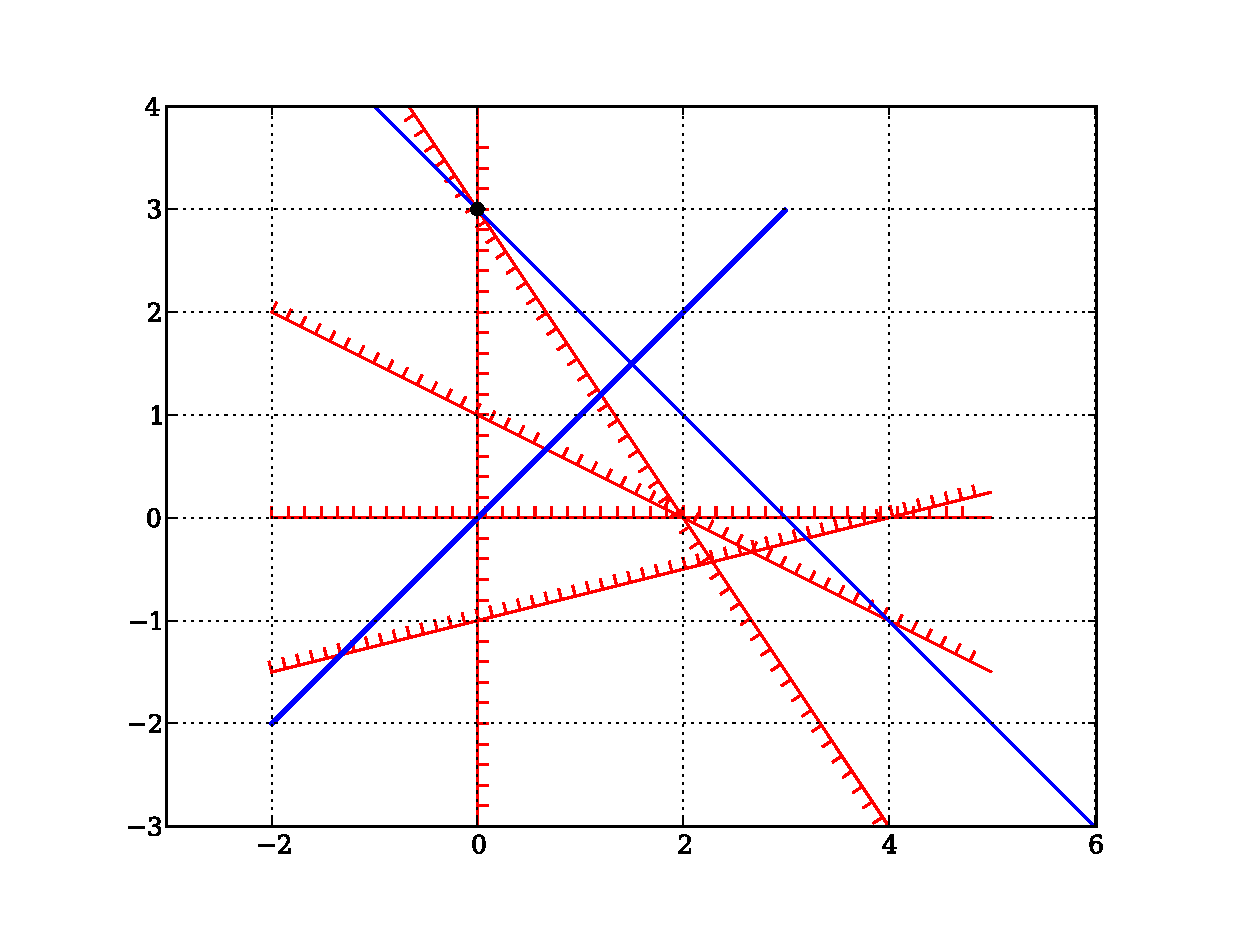
\includegraphics[width=\textwidth]{img/31}
\caption{Решение графическим методом}\label{31}
\end{figure}
